
% ===============================================
% MATH 34: Multivariable calculus           Spring 2019
% hw_template.tex
% ===============================================

% -------------------------------------------------------------------------
% You can ignore this preamble. Go on
% down to the section that says "START HERE" 
% -------------------------------------------------------------------------

\documentclass{article}

\usepackage[margin=1.5in]{geometry} % Please keep the margins at 1.5 so that there is space for grader comments.
\usepackage{amsmath,amsthm,amssymb,hyperref}
\usepackage{graphicx}
\usepackage{float}
\usepackage{listings}
\usepackage{xparse}
\usepackage{xcolor}
\usepackage{verbatim}

\newcommand{\R}{\mathbf{R}}  
\newcommand{\Z}{\mathbf{Z}}
\newcommand{\N}{\mathbf{N}}
\newcommand{\Q}{\mathbf{Q}}
\newcommand{\C}{\mathbf{C}}
\newcommand{\Log}{\text{Log}}
\newcommand{\Arg}{\text{Arg}}
\newcommand{\Real}{\text{Re}}
\newcommand{\Imag}{\text{Im}}
\newcommand{\ddz}{\frac{d}{dz}}

\newenvironment{theorem}[2][Theorem]{\begin{trivlist}
\item[\hskip \labelsep {\bfseries #1}\hskip \labelsep {\bfseries #2.}]}{\end{trivlist}}
\newenvironment{lemma}[2][Lemma]{\begin{trivlist}
\item[\hskip \labelsep {\bfseries #1}\hskip \labelsep {\bfseries #2.}]}{\end{trivlist}}
\newenvironment{claim}[2][Claim]{\begin{trivlist}
\item[\hskip \labelsep {\bfseries #1}\hskip \labelsep {\bfseries #2.}]}{\end{trivlist}}
\newenvironment{problem}[2][Problem]{\begin{trivlist}
\item[\hskip \labelsep {\bfseries #1}\hskip \labelsep {\bfseries #2.}]}{\end{trivlist}}
\newenvironment{proposition}[2][Proposition]{\begin{trivlist}
\item[\hskip \labelsep {\bfseries #1}\hskip \labelsep {\bfseries #2.}]}{\end{trivlist}}
\newenvironment{corollary}[2][Corollary]{\begin{trivlist}
\item[\hskip \labelsep {\bfseries #1}\hskip \labelsep {\bfseries #2.}]}{\end{trivlist}}

\newenvironment{solution}{\begin{proof}[Solution]}{\end{proof}}

\makeatletter
\newcommand{\skipitems}[1]{%
	\addtocounter{\@enumctr}{#1}%
}
\makeatother

\NewDocumentCommand{\codeword}{v}{%
\texttt{\textcolor{blue}{#1}}%
}


\begin{document}

\large % please keep the text at this size for ease of reading.

% ------------------------------------------ %
%                 START HERE             %
% ------------------------------------------ %

{\Large Page 1 % Replace with appropriate page number 
\hfill  MTH483, Complex Variables, HW5}

\begin{center}
{\Large Wyatt Whiting}
\end{center}
\vspace{0.05in}

% -----------------------------------------------------
% The "enumerate" environment allows for automatic problem numbering.
% To make the number for the next problem, type " \item ". 
% To make sub-problems such as (a), (b), etc., use an "enumerate" within an "enumerate."
% -----------------------------------------------------
\begin{enumerate}

	\item Evaluate the following limits.
	\begin{enumerate}
		\item 
		\[\lim_{z\to i}\frac{z^3+i}{z-i} =  \lim_{z\to i}\frac{3z^2}{1}\text{ (by L'Hopital's Rule ) }=\frac{3(-1)}{1}=-3.\]
		\item 
		\[\lim_{z\to 0}\frac{\Log(z+i)-\Log(i)}{z} =  \lim_{z\to 0}\frac{\Log(z+i)-\frac{i\pi}{2}}{z} = \text{ (L'H) }\lim_{z\to 0}\frac{\frac{1}{z+i}}{1}= \]
		\[\lim_{z\to 0}\frac{1}{z+i}=\frac{1}{i}=-i \]
		\item 
		\[\lim_{z\to 0}\frac{e^z-1}{\Log(z+1)}=\text{ (L'H) } \lim_{z\to 0}\frac{e^z}{\frac{1}{z+1}} =\lim_{z\to 0}e^z(z+1)=1(1)=1 \]
		
		
		\item 
		\[ \lim_{z\to\infty}z\sin\left(\frac{1}{z}\right), w=1/z \]
		\[\lim_{z\to\infty}1/z = \lim_{z\to\infty}w=0=\lim_{w\to 0}w \implies \lim_{z\to\infty}f(1/z)=\lim_{w\to 0}f(w)\]
		\[\lim_{w\to 0}\frac{\sin(w)}{w}=\text{ (L'H) } =\lim_{w\to 0}\frac{\cos(w)}{1}=1\]
	\end{enumerate}
	
	\item Consider the function $f(z)=z/|z|$, where $z=x+yi$. 
	\begin{enumerate}
	
		\item 
		\[f(a+bi)=\left(\frac{x}{\sqrt{x^2+y^2}}\right)+i\left(\frac{y}{\sqrt{x^2+y^2}}\right)\]
		
		\item Use Mathematica to plot $u$ and $v$.
		\codeword{Plot3D[Re[(x + I y)/Abs[x + I y]], {x, -5, 5}, {y, -5, 5}]}
		\begin{figure}[H]
		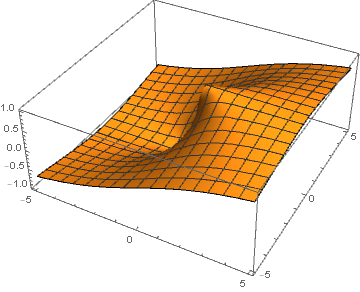
\includegraphics[scale=0.8]{image1.png}
		\end{figure}
		This is the real component of $f(z)$
		\codeword{Plot3D[Im[(x + I y)/Abs[x + I y]], {x, -5, 5}, {y, -5, 5}]}
		\begin{figure}[H]
		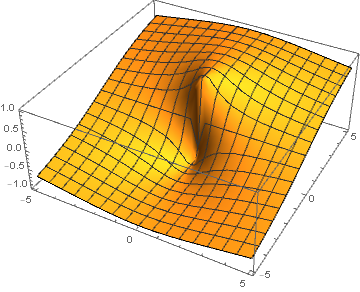
\includegraphics[scale=0.8]{image2.png}
		\end{figure}
		This is the imaginary component of $f(z)$.
		\begin{figure}[H]
		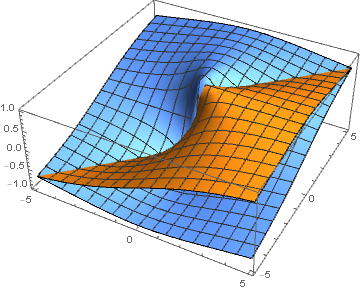
\includegraphics[scale=0.8]{image3.png}
		\end{figure}
		Here are the two figures in the same graph, where the real is in orange and the imaginary in blue.
		
		\item Find the limit of $f(z)$ as $z$ approaches 0 along each of the following paths:
		\begin{enumerate}
			\item \[ \lim_{t\to 0^{\text{-}}}f(t+0i)=\lim_{t\to 0^{\text{-}}}\frac{t}{\sqrt{t^2}} = \lim_{t\to 0^{\text{-}}}\frac{t}{|t|} = -1\]
			\item \[ \lim_{t\to 0^{\text{+}}}f(t+0i)=\lim_{t\to 0^{\text{+}}}\frac{t}{\sqrt{t^2}} = \lim_{t\to 0^{\text{+}}}\frac{t}{|t|} = 1\]
			\item \[ \lim_{t\to 0^{\text{-}}}f(0+ti)=\lim_{t\to 0^{\text{-}}}i\frac{t}{\sqrt{t^2}} = \lim_{t\to 0^{\text{-}}}i\frac{t}{|t|} = -i\]
			\item \[ \lim_{t\to 0^{\text{+}}}f(0+ti)=\lim_{t\to 0^{\text{+}}}i\frac{t}{\sqrt{t^2}} = \lim_{t\to 0^{\text{+}}}i\frac{t}{|t|} = i\]
		\end{enumerate}
		
		\item Find the limit of $f(z)$ as $z$ approaches $\infty$ along each of the following paths:
		\begin{enumerate}
			\item \[ \lim_{t\to\infty}f(t+0i)=\lim_{t\to\infty}\frac{t}{\sqrt{t^2}}=\lim_{t\to\infty}\frac{t}{|t|}=1 \]
			\item \[ \lim_{t\to\infty}f(0+ti)=\lim_{t\to\infty}i\frac{t}{\sqrt{t^2}}=\lim_{t\to\infty}i\frac{t}{|t|}=i \]
		\end{enumerate}
		
	\end{enumerate}	
	
	\item $f(z)=\Log(z)=\ln|z|+i\Arg(z) \implies u = \ln|z| \text{ and } v = \Arg(z)$. To satisfy the Cauchy-Riemann equations, it must be the case that:
	\[\frac{\partial \ln|z|}{\partial x} = \frac{1}{z}= \frac{\partial \Arg(z)}{\partial y} \text{   (1)}\]
	
	\[\frac{\partial \ln|z|}{\partial y}=\frac{i}{z}=-\frac{\partial \Arg(z)}{\partial x} \text{   (2)}\]
	
	\[\text{(1)}\implies  \frac{1}{x+iy}=\frac{x-iy}{x^2+y^2}=
		\begin{cases}
			\frac{x}{x^2+y^2} & \text{if $x>0$} \\
			\frac{xy}{\sqrt{\frac{y^2}{x^2+y^2}}(x^2+y^2)^{3/2}} & \text{if $y>0$} \\
			-\frac{xy}{\sqrt{\frac{y^2}{x^2+y^2}}(x^2+y^2)^{3/2}} & \text{if $y<0$}
		\end{cases}
	\]
	
	\[\implies \frac{x}{x^2+y^2}=\frac{x}{x^2+y^2} \text{ when $x>0$.}\]
	
	\[\frac{x}{x^2+y^2}=\frac{xy}{\sqrt{\frac{y^2}{x^2+y^2}}(x^2+y^2)^{3/2}} \implies 1 = \frac{y}{\sqrt{\frac{y^2}{x^2+y^2}}\sqrt{x^2+y^2}}=\frac{y}{\sqrt{y^2}}=\frac{y}{|y|}, \]
	
	\[\text{so }1 = \frac{y}{|y|}\text{ when $y>0$. Since $x\leq 0$  and $y\neq 0$, then this excludes}\{z=t+0i:t\in\R_{\leq 0}\}\]
	
	\[\frac{x}{x^2+y^2}=-\frac{xy}{\sqrt{\frac{y^2}{x^2+y^2}}(x^2+y^2)^{3/2}} \implies 1 = -\frac{y}{\sqrt{\frac{y^2}{x^2+y^2}}\sqrt{x^2+y^2}}=-\frac{y}{\sqrt{y^2}}=-\frac{y}{|y|} \]
	
	\[\text{so }1 = -\frac{y}{|y|}\text{ when $y<0$, which excludes the same region as above.}\]
	Thus the first half of the Cauchy-Riemann equation is satisfied on $\C\setminus\R_{\leq 0}$
	
	\[\text{(2)}\implies  \frac{i}{x+iy}=\frac{y+ix}{x^2+y^2}=
		\begin{cases}
			\frac{y}{x^2+y^2} & \text{if $x>0$} \\
			\frac{\sqrt{\frac{y^2}{x^2+y^2}}}{\sqrt{x^2+y^2}} & \text{if $y>0$} \\
			-\frac{\sqrt{\frac{y^2}{x^2+y^2}}}{\sqrt{x^2+y^2}} & \text{if $y<0$}
		\end{cases}
	\]
	
	\[\implies \frac{y}{x^2+y^2}=\frac{y}{x^2+y^2} \text{ when $x > 0$} \]
	
	\[\frac{y}{x^2+y^2}=\frac{\sqrt{\frac{y^2}{x^2+y^2}}}{\sqrt{x^2+y^2}}=\frac{|y|}{x^2+y^2}\text{ when $y > 0$} \]
	
	This excludes $z=0+0i$ since this point causes a division-by-zero error.
	
	\[\frac{y}{x^2+y^2}=-\frac{\sqrt{\frac{y^2}{x^2+y^2}}}{\sqrt{x^2+y^2}}=-\frac{|y|}{x^2+y^2}\text{ when $y < 0$}. \]
	This excludes the origin, just as above.
	
	Therefore, the Cauchy-Riemann equations are satisfied on $\C\setminus\R_{\leq 0}$. It then follows that $f(z)=Log z$ is holomorphic on $\C\setminus\R_{\leq 0}$.
	
	
	\item 
	
	\[ F(z)=z\Log(z)-z\]
	\[F'(z)=\frac{d}{dz}[z\Log(z)-z]=\frac{d}{dz}[z\Log(z)]-\frac{d}{dz}[z] \]
	\[=\ddz[z]\Log(z)+z\ddz[\Log(z)]-1=\Log(z)+z\ddz[Log(z)-1] \]
	We now apply chain rule. $\ddz[Log(z)]=\frac{d\Log(u)}{du}\frac{du}{dz}$ where $u=z$ and $\frac{d}{du}[Log(u)]=\frac{1}{u}$, giving
	
	\[=\Log(z)+z\frac{\ddz[z]}{z}-1=\Log(z)+z\frac{1}{z}-1=\Log(z)+1-1=\Log(z). \]
	This shows that $F'(z)=\Log(z)=f(z) \implies F(z)$ is an antiderivative of $f(z)$
	
	\item Consider the function $f(z)=\Log(z)+
	\Log(iz-i)$
	\begin{enumerate}
		\item We know that $\Log(z)$ on its own is holomorphic on $\C\setminus\R_{\leq 0}$. Next we know $\Log(iz+i)=\Log(i(z-1))$. So we must exclude from the region of holomorphism all $i(z-1)=-a+0i \implies z-1 =0+ia \implies z = 1 + ia$ where $a\geq 0$. This shows we have to remove $\{z=1+ia\in\C :  a\geq 0\}$ from the region of holomorphism on $\C$. We may then conclude that $f(z)=\Log(z)+\Log(iz+i)$ is $\C\setminus (\R_{\leq 0} \cup \{z=1+ia\in\C :  a\geq 0\})$
		\item Determine all antiderivatives on the region $\C\setminus\R_{\leq 0}$
		\[\int f(z)dz=\int \Log(z)+\Log(iz-i)dz=\int \Log(z)dz+\int \Log(iz-i)dz\]
		\[ =[z\Log(z)-z+c_1]+[z\Log(iz-i)-z-\Log(1-z)+c_2] \]
		\[=z(\Log(z)+\Log(iz-i)-2)-\Log(1-z)+c \]
		\[\text{ where }c = c_1+c_2 \text{ is an arbitrary constant.}\]
	\end{enumerate}
	
	\item The upper semicircle $C_2(0)$ oriented counter-clockwise is parametrized by 
	$$\gamma := 2\cos(t)+2 i\sin(t)=2e^{it},t\in [0, \pi]$$
	\[\gamma' := -2\sin(t)+2i\cos(t)=2ie^{it} \]
	\begin{enumerate}
		\item $f(z)=z+\overline{z}=a+bi+(a-bi)=2a=2\Real(z)$
		\[ \int_{\gamma} f(z) dz = \int_{0}^{\pi}f(2\cos(t)+2 i\sin(t))(-2\sin(t)+2i\cos(t))dt\]
		\[=\int_{0}^{\pi}4\cos(t)(-2\sin(t)+2i\cos(t)) dt=\int_{0}^{\pi}-8\cos(t)\sin(t)+8i\cos^2(t) dt\]
		\[=8\int_{0}^{\pi}\cos(t)\sin(t)+8i\int_{0}^{\pi}\cos^2(t)dt=0+8i\left[\frac{\pi}{2}\right]=4i\pi\]
		\item $f(z)=z^2-2z+3$
		
		\[ \int_{\gamma} f(z) dz = \int_{0}^{\pi}f(2e^{it})2ie^{it}dt=\int_{0}^{\pi}((2e^{it})^2-4e^{it}+3)(2ie^{it})dt\]
		\[ \int_{0}^{\pi}(2e^{2it}-4e^{it}+3)(2ie^{it})dt=\int_{0}^{\pi}4ie^{3it}-8ie^{2it}+6ie^{it}dt\]
		\[=\left[ \frac{4}{3}e^{3it}-4e^{2it}+6e^{it}  \right]_{0}^{\pi} =\left( -\frac{4}{3}-4-6\right)-\left(\frac{4}{3}-4+6\right)\]
		\[ =-\frac{8}{3}-12=-\frac{44}{3}\]
		
		\item $f(z)=xy=\Real(z)\Imag(z)$
		\[ \int_{\gamma} f(z) dz = \int_{0}^{\pi}f(2\cos(t)+2 i\sin(t))(-2\sin(t)+2i\cos(t))dt\]
		\[=\int_{0}^{\pi}(4\cos(t)\sin(t))(-2sin(t)+2i\cos(t))dt \]
		\[= -8\int_{0}^{\pi}\cos(t)\sin^2(t)dt+8i\int_{0}^{\pi}\cos^2(t)\sin(t)dt \]
		\[=0+8i\left[ -\frac{1}{3}\cos^3(t)\right]_{0}^{\pi}=\frac{16i}{3} \]
		
		\item $f(z)=\frac{1}{z^4}=z^{-4}$
		
		\[\int_{\gamma}f(z)dz=\int_{0}^{\pi}f(2e^{it})(2ie^{it})dt =\int_{0}^{\pi}(2e^{it})^{-4}(2ie^{it}) \]
		\[=\int_{0}^{\pi}2e^{-4it}(2ie^{it})dt=\int_{0}^{\pi}4ie^{-3it}dt=\left[-\frac{4}{3}e^{-3it} \right]_{0}^{\pi} \]
		\[ =\frac{4}{3}+\frac{4}{3}=\frac{8}{3} \]
	\end{enumerate}
\end{enumerate}

% ---------------------------------------------------
% Anything after the \end{document} will be ignored by the typesetting.
% ----------------------------------------------------

\end{document}

